\documentclass[conference]{IEEEtran}
\IEEEoverridecommandlockouts

\usepackage{cite}
\usepackage{amsmath,amssymb}
\usepackage{graphicx}
\usepackage{textcomp}
\usepackage{booktabs}
\usepackage[hidelinks]{hyperref}

%% =================================================================
%% FLOAT PLACEMENT -- keeps every figure next to the text that cites
%% it instead of letting LaTeX defer them to the last pages.
%% =================================================================
\usepackage{stfloats}          % lets a figure* sit at the bottom of a page
\renewcommand{\topfraction}{0.92}
\renewcommand{\bottomfraction}{0.85}
\renewcommand{\textfraction}{0.07}
\renewcommand{\floatpagefraction}{0.75}
\renewcommand{\dbltopfraction}{0.92}
\renewcommand{\dblfloatpagefraction}{0.75}
\setcounter{topnumber}{3}
\setcounter{bottomnumber}{2}
\setcounter{totalnumber}{4}
\setcounter{dbltopnumber}{2}

%% =================================================================
%% PAGE FIT -- tightened float/caption spacing to hold 6 pages.
%% If the paper still runs to 7, uncomment the knobs in order:
%%   1. \setlength{\parskip}{-0.2pt}
%%   2. shrink fig:hardware to 0.92\columnwidth
%%   3. add \footnotesize just after \begin{thebibliography} (see References)
%% =================================================================
\setlength{\textfloatsep}{8pt plus 2pt minus 2pt}
\setlength{\floatsep}{8pt plus 2pt minus 2pt}
\setlength{\intextsep}{8pt plus 2pt minus 2pt}
\setlength{\dblfloatsep}{8pt plus 2pt minus 2pt}
\setlength{\dbltextfloatsep}{8pt plus 2pt minus 2pt}
\setlength{\abovecaptionskip}{4pt}
\setlength{\belowcaptionskip}{0pt}

\begin{document}

\title{Measuring the Urban-to-Wilderness Domain Gap in\\
Aerial Person Detection on Raspberry Pi 4 Hardware}

\maketitle

\begin{abstract}
The only aerial corpora large enough to train a person detector are urban
traffic surveillance, while the missions that matter are flown over wilderness.
Almost every published accuracy figure in this field is measured in-domain, so
the cost of that mismatch is unknown. We train tiled nano-scale detectors on
VisDrone and evaluate them zero-shot on WiSARD, a wilderness corpus of 37,058
tiles from 38 flight sequences, with intervals resampled over sequences. Person
detection falls from 0.3997 to 0.2567 AP@0.5. A resize-only control scored with
inference-time slicing reaches 0.0449, bounding the gain from training-time
tiling at 5.7$\times$. Contrary to the usual small-object framing, wilderness
targets are three times larger than the training distribution and are viewed
from nadir. Halving the inference input recovers 0.068 AP@0.5, but by
suppressing 46\% of false positives rather than by finding more people. Two
training-time factors are hidden by in-domain evaluation: cross-domain accuracy
is not monotone in training, peaking near epoch 70 and falling by roughly a
sixth while in-domain validation still rises, so the gap we report is an upper
bound. Raising the negative-tile fraction from 1.33\% to 9.55\% cuts false
positives by a third at mid-range matched recall, though not at every level.
Fine-tuning recovers a factor of 6.1, saturating near sixteen labelled
sequences, and repeated coverage lifts encounter-level detection from 0.609 to
0.923. Throughput is measured on a Raspberry Pi 4 without non-maximum
suppression, so it bounds deployed cost from below; no result here is
flight-validated.
\end{abstract}

\begin{IEEEkeywords}
aerial person detection, search and rescue, domain shift, small-object
detection, edge inference, unmanned aerial vehicles
\end{IEEEkeywords}

\section{Introduction}

Search and rescue is a race against time, and the ground to cover is often too
large or too dangerous for a walking team. A small quadcopter with a camera
sweeps the same ground in a fraction of the time, reaches terrain a team on foot
cannot, and returns imagery a coordinator can act on, if its onboard computer is
cheap enough to afford, and a Raspberry Pi 4 costs a fraction of a Jetson-class
board while drawing a few watts. Prior work has flown this hardware class, in
Pixhawk-based Pi 4 payloads, low-cost detection and geolocation pipelines, and
an ArduPilot avalanche search drone \cite{elashaal2024,lago2024,stasik2025},
cited here for the hardware class, not as baselines. We assembled a payload of
the same class around a Pixhawk 2.4.8 and a Raspberry Pi 4
(Fig.~\ref{fig:hardware}) as the deployment target, though every measurement
below is made on recorded imagery and on that Pi 4 on a desk.

The main difficulty for such a platform is not model capacity, it is data: the
only aerial datasets large enough to train a person detector are urban
traffic-surveillance corpora, while the missions that matter are flown over
wilderness. A detector must be trained in one visual domain and flown in
another, and the literature says little about what that costs, because almost
every published search-and-rescue detection number is measured in-domain. A
thermal camera beats a visible one here, at 0.977 against 0.892 mAP@0.5 on the
same scenes; we work in RGB because payload, cost and power leave this airframe
class little choice, and the visible-spectrum gap decides whether thermal is
worth buying.

Three kinds of prior work touch this problem, and each stops short of it. Tiled
inference such as SAHI \cite{akyon2022} rescues small targets but is reported as
an inference-time wrapper, measured in-domain. Cross-domain drops have been
measured for aerial detectors \cite{chen2026,song2025,sambolek2024}, but as
single before-and-after numbers, and edge quantisation studies report the speed
and accuracy trade on Pi-class hardware \cite{ahn2023,rey2025}, but for
detectors that never leave their training domain. No study connects the three.

This paper makes that measurement, training tiled nano-scale detectors on
VisDrone, a three-class urban aerial corpus, and evaluating them zero-shot on
WiSARD, a wilderness corpus of 37,058 tiles from 38 flight sequences. Person
AP@0.5 falls from 0.3997 in-domain to 0.2567 across domains, and the shift is
not the one usually assumed: WiSARD persons are larger and seen from nadir. The
main contributions are:

\begin{itemize}
\item A sequence-resampled measurement of the urban-to-wilderness gap for a
Pi-class detector, and a characterisation of the shift as one toward larger,
nadir targets, without ranking the size and viewpoint components
(Sections~\ref{sec:method} and \ref{sec:results}).

\item Evidence that tiled training preserves most of what survives the domain
change, worth at most 5.7$\times$ over a resize-only control, and that halving
the inference input recovers 0.068 AP@0.5 by suppressing 46\% of false
positives rather than finding people (Section~\ref{sec:results}).

\item Two training-time effects the in-domain view hides: cross-domain accuracy
peaks near epoch 70 then falls by a sixth while in-domain validation rises, and
extra negative tiles cut false positives at mid-range matched recall by a third
(Section~\ref{sec:discussion}).

\item A bound on what target data buys: fine-tuning recovers a factor of 6.1,
saturating near sixteen labelled sequences (Section~\ref{sec:results}).
\end{itemize}

Section~\ref{sec:related} reviews prior work, Section~\ref{sec:method} the
corpora, platform, pipeline and metrics, Section~\ref{sec:results} the results,
Section~\ref{sec:discussion} their interpretation, Section~\ref{sec:limits}
their bounds, and Section~\ref{sec:conclusion} concludes.

\section{Related Work}
\label{sec:related}

\subsection{Aerial Person Detection for Search and Rescue}

Nano-scale YOLO variants are the practical standard for onboard detection
\cite{humes2023,alqahtani2024}, from drowning-swimmer detection \cite{zell2026}
to a thirty-three-model sweep across RGB/LWIR fusion ratios \cite{sachdeva2025}.
A recent survey finds most aerial personnel objects under twenty pixels and
in-domain VisDrone pedestrian accuracy below 50\% \cite{zhang2025}. We train on
VisDrone \cite{zhu2021} and evaluate on WiSARD \cite{broyles2022}.

Two properties of this literature affect how its numbers should be read. First,
published results are overwhelmingly in-domain: the WiSARD visual baseline of
0.892 mAP@0.5 was measured after removing every tile with no person from both
training and test, removing most chances for a false positive. Second, the
protocol is worth more than many method contributions \cite{manzini2023}. The
same detector scores AP 80.1 under VOC2012 and 91.5 under SAR-APD, and one
recent system counts a detection correct at IoU 0.20 and selects on F1
\cite{fraternali2025}. Our numbers use a strict COCO-style IoU 0.5 over every
tile, including the 85.8\% with no person. That has a measurable cost. Rescoring
one fixed detection set under the corpus authors' positives-only protocol raises
AP@0.5 from 0.257 to 0.329, because 77.1\% of our detections fall on the 31,793
empty tiles that protocol discards. Protocol thus accounts for 11.3\% of the
apparent distance to 0.892; the remaining 0.563 is domain shift.

\subsection{Tiling and Small-Object Inference}

Resizing a high-resolution aerial frame to a detector's input destroys small
targets before the network sees them. Slicing the frame instead is the
established remedy. SAHI \cite{akyon2022} formalises it and reports AP gains of
5--7\% from sliced inference alone, more with slicing applied during
fine-tuning. A stride-4 detection level attacks the same problem
architecturally, lifting mAP@0.5 from 0.786 to 0.849 at unchanged parameter
count \cite{chen2026}. We adopt tiling at training time rather than as an
inference-only wrapper, and treat the untiled resize as a control.

\subsection{The Cross-Domain Gap}

Where cross-domain transfer has been measured in aerial detection, the drops are
large and consistent. One study reports mAP@0.5 falling from 0.786 in-domain to
0.377--0.398 on an unseen corpus \cite{chen2026}, and another observes 0.94 to
0.32 for an aerial infrared detector moved between two infrared datasets
\cite{song2025}. The most directly comparable pair comes from
\cite{sambolek2024}. YOLOv8n scores mAP@0.5 of 35.9 transferred from COCO to the
SARD wilderness corpus and 86.8 after fine-tuning, a gap the authors attribute
to SARD's bird's-eye view. A deployed aerial-ground search system fine-tunes
YOLOv11 on VisDrone with class remapping \cite{farrell2025}, a precedent for our
training corpus, and domain adaptation is named as one of four open challenges
for the field \cite{zhang2025}. Those studies report the gap as a single
before-and-after number; this paper decomposes it into what tiling preserves,
what inference resolution recovers, what schedule and negative sampling
contribute, and what target-domain data closes, for a detector that fits a
Pi~4.

\subsection{Quantisation on Raspberry Pi Class Hardware}

Integer quantisation trades accuracy for speed on CPU-class hardware
\cite{jacob2018,wu2020,gholami2022}. A Raspberry Pi ARM CPU sees a 2.61$\times$
INT8 speedup with no accuracy loss except under static quantisation
\cite{ahn2023}, the scheme an edge deployment would use. The detector case is
harsher. YOLOv8n loses 13.5 points of mAP@0.5 from FP16 to INT8 against 5.8 for
YOLOv8s \cite{rey2025}, and INT8 YOLOv4-tiny runs on a Pi 5 at 28.2\,ms and
13.85\,W \cite{boddu2025}. We reproduce the nano-scale result on a Pi 4 and
locate the loss in the integer-activation path.

\begin{figure*}[!t]
\centering
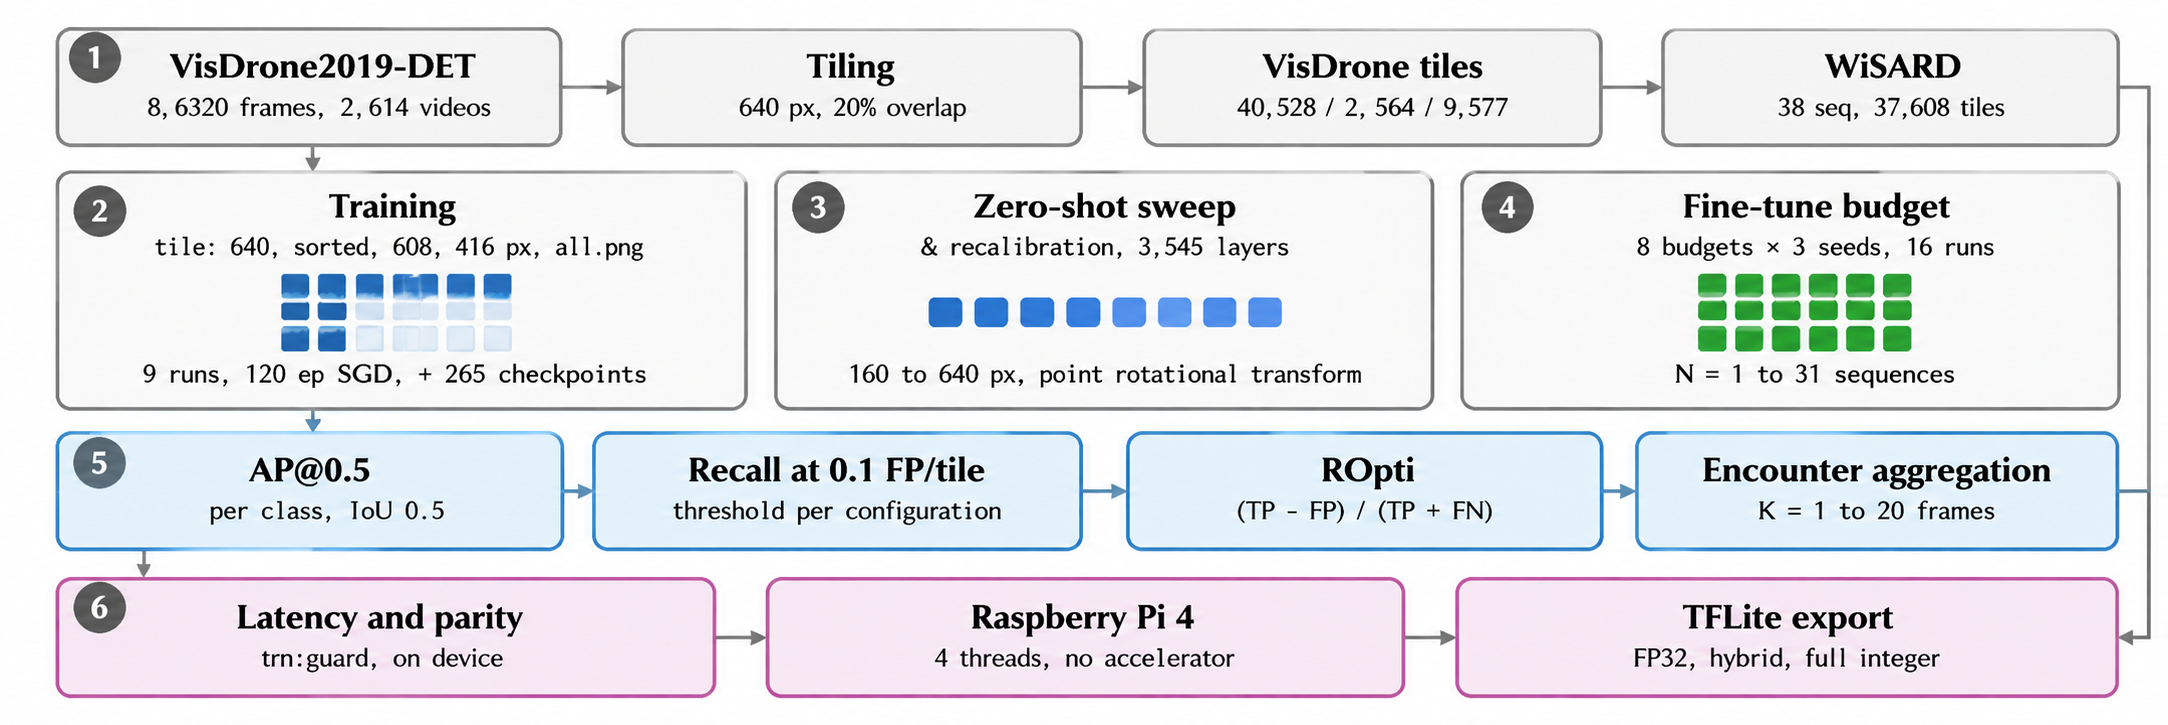
\includegraphics[width=17cm,height=7cm]
{fig1_pipeline.png}
\caption{The measurement pipeline, numbered by its five stages. Each chip is one
run, and the pale cells in the training grid mark the three configurations that
ran at one seed rather than three. The on-device branch is fed from the trained
checkpoint, not from the metrics above it. Every count is read from the
committed result files.}
\label{fig:pipeline}
\end{figure*}

\section{Method}
\label{sec:method}

\subsection{Problem Setting}

A rescue team flies a consumer-class quadcopter with a visible-spectrum camera
at 20--120\,m over wilderness. The onboard computer is a Raspberry Pi 4 with no
accelerator. The detector must be trained on public data, because no wilderness
corpus is large enough to train from. Everything below is measured on recorded
imagery and on a Pi 4 on a desk (Fig.~\ref{fig:pipeline}).

\begin{figure}[!t]
\centering
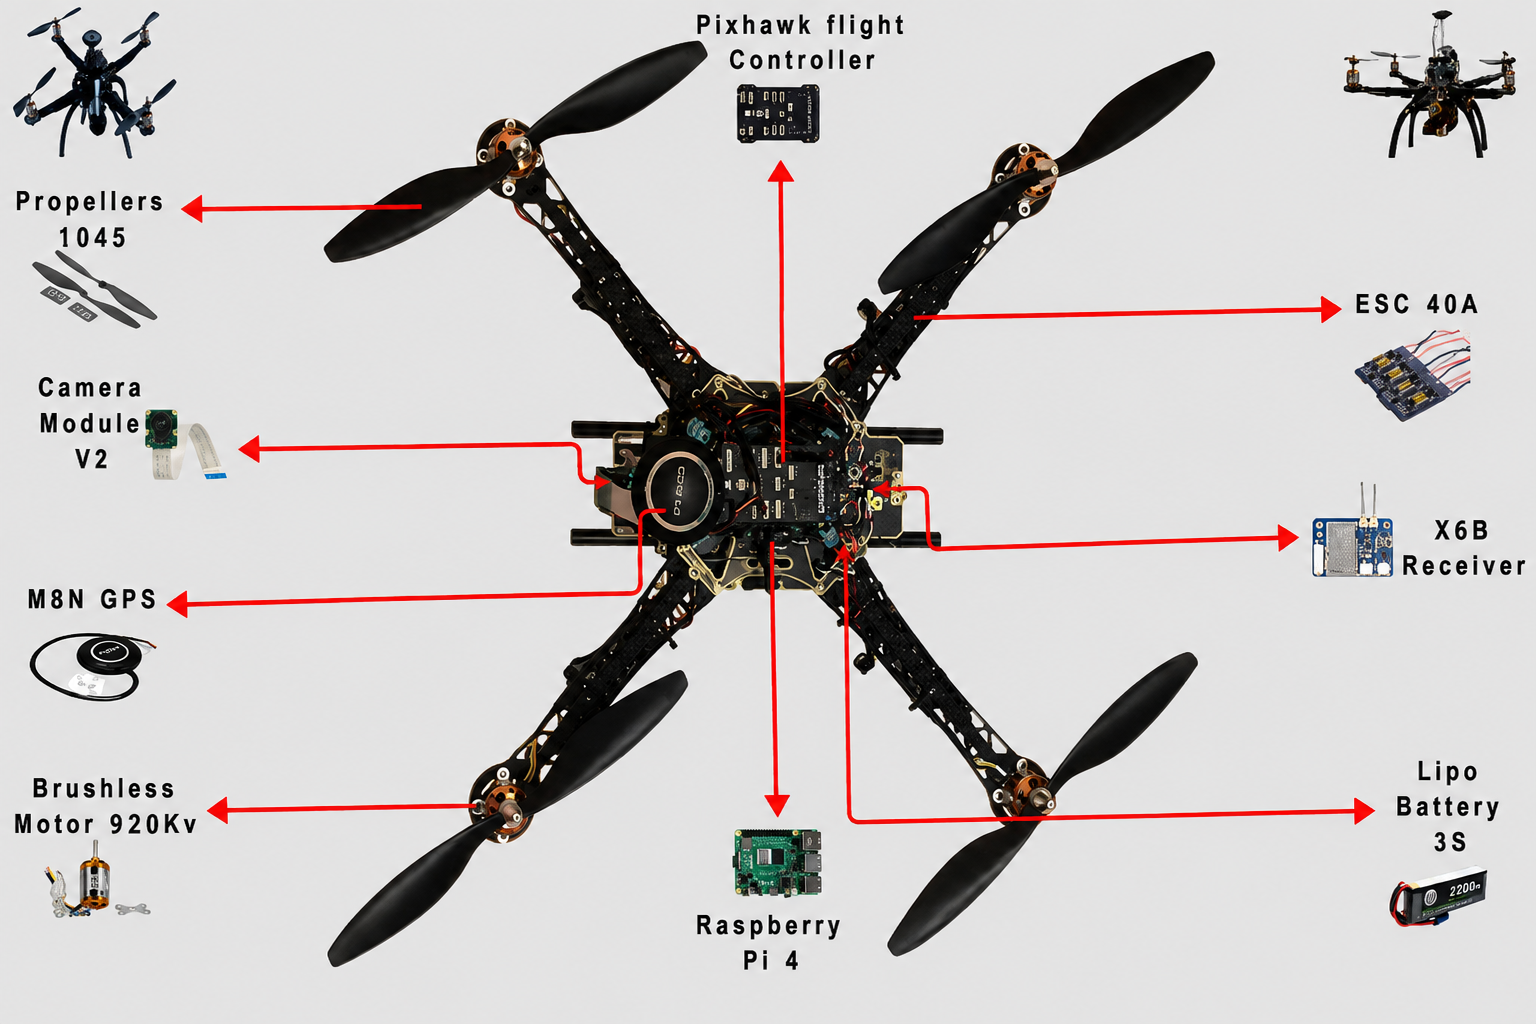
\includegraphics[width=\columnwidth]
{fig2_hardware.png}
\caption{The assembled quadcopter and its labelled components: Pixhawk flight
controller, Raspberry Pi 4, Camera Module V2, M8N GPS, X6B receiver, 40\,A ESC,
1045 propellers, 920\,Kv brushless motor and 3S LiPo battery.}
\label{fig:hardware}
\end{figure}

\subsection{Target Platform}

The detector is intended for a quadcopter we assembled for this purpose.
Fig.~\ref{fig:hardware} shows the airframe and its labelled components: a
Pixhawk 2.4.8 flight controller, a Raspberry Pi 4 companion computer, a Camera
Module V2, an M8N GPS, an X6B receiver, 40\,A ESCs, 920\,Kv brushless motors,
1045 propellers and a 3S LiPo battery. The Pi 4 is the only compute on board and
carries no accelerator, which is what fixes the latency budget of
Section~\ref{sec:ondevice}. The platform defines the deployment target and is
not itself part of the measurement: every accuracy figure below comes from
recorded imagery and every latency figure from a Pi 4 on a desk, so nothing
reported here is flight-validated (Section~\ref{sec:limits}).

\subsection{Corpora and Label Space}

Training used VisDrone2019-DET \cite{zhu2021}, an urban aerial corpus of 8,629
annotated frames in the official 6,471/548/1,610 train/validation/test-dev
partition, from 208, 76 and 61 video sequences. Its ten categories were
collapsed to the three a search-and-rescue operator acts on (person, vehicle,
two-wheeler), giving 343,205, 38,759 and 75,102 instances per split; categories
outside the mapping were discarded, not merged into a background class.

Cross-domain evaluation used WiSARD \cite{broyles2022}, a wilderness corpus
recorded from consumer airframes at 20--120\,m. We used its visible-spectrum
subset at every tenth frame, giving 2,586 frames across 38 sequences. WiSARD is
annotated for person only, so we declare it in the same three-class space and
report the person row exclusively; any correct vehicle detection would otherwise
count as a false positive against absent ground truth.

Frames within one flight are near-duplicates, so a frame-level partition
inflates accuracy, and all partitions are made at sequence granularity. The
converted VisDrone layout restarts video identifiers per split, so we parse the
identifier from the filename and namespace it by split; MD5 hashing over all
8,629 images found zero cross-split duplicates.

\subsection{Tiling}

Tiling is applied when the dataset is built, not only at inference, because
resizing destroys small targets before training as well as before detection.
Each frame was cut into overlapping 640\,px tiles at native resolution with 20\%
overlap, the final tile in each row and column flushed to the far edge. A
ground-truth box was kept for a tile when at least 30\% of its area fell inside.
All positive tiles were kept and negatives subsampled at 17.5\% per frame,
giving 40,523, 2,784 and 9,377 tiles. Applied per frame, that fraction rounds
away most frames' few empty tiles, so the realised composition is 1.33\%
negative, not the 15--20\% intended. As a control, an otherwise identical model
was trained on whole frames resized to the same input.

The class balance differs sharply between the corpora, and it matters below. Of
the 40,523 VisDrone training tiles, 39,983 (98.7\%) contain at least one
annotated object; of the 37,058 WiSARD tiles, only 5,265 (14.2\%) contain a
person.

\subsection{Training}

We trained YOLO11n and YOLOv8n for 120 epochs at 640\,px with batch 32, and one
YOLO11n variant at 416\,px with batch 48, all under SGD with a cosine schedule,
early-stopping patience of 25, deterministic kernels at seed 42, and
COCO-pretrained initialisation, on a single 8\,GB RTX 3060 Ti. The two headline
configurations were replicated at seeds 123 and 456.

\subsection{Target-Domain Fine-Tuning}

To bound what target-domain data recovers, the WiSARD tiles were partitioned
into sequence-disjoint train, validation and test sets. Allocation balanced
annotated person boxes rather than tile counts, since six of the 38 sequences
contain no person and per-sequence box counts range from 0 to 1,122, so a
tile-balanced split can put almost every person on one side while looking even.
The realised split holds 31, 2 and 5 sequences with 5,685, 1,161 and 1,499
boxes, or 68.1/13.9/18.0\% of the annotated people. Fine-tuning initialised from
the VisDrone-trained tiled 640\,px checkpoint under SGD at a reduced learning
rate of $10^{-3}$. Validation accuracy peaked at epoch 5 and did not improve
over the next sixteen, so we report the epoch-5 checkpoint.

\subsection{Metrics and Uncertainty}

Detections were matched greedily in descending confidence at IoU 0.5, each
ground-truth box consumable once so duplicates count as false positives, and
average precision is all-point interpolated. Because a missed person costs far
more than a dismissed false alarm, we also report recall at a fixed budget of
0.1 false positives per tile, with the threshold that achieves it. Generic
metrics understate the operational cost of false alarms here \cite{manzini2023},
so we additionally report
$\mathrm{ROpti}=(\mathrm{TP}-\mathrm{FP})/(\mathrm{TP}+\mathrm{FN})$
\cite{sambolek2024}, unbounded below and threshold-dependent; we give it at the
operating point above and at its own maximum, naming the threshold each time.

Confidence intervals resample sequences, not tiles or boxes. WiSARD tiles come
from consecutive video and are strongly correlated within a flight, so a
tile-level bootstrap would treat near-duplicates as independent and return an
indefensibly narrow interval. All intervals are 10,000-resample percentile
intervals over the 38 sequences; where two configurations are compared, both are
scored on the same resampled sequences and the interval is taken on their
difference, the right test for a paired comparison.

\subsection{On-Device Measurement}
\label{sec:ondevice}

Deployment measurements were taken on the Raspberry Pi 4 under TensorFlow Lite
with four threads, discarding 60 warm-up iterations before 160 timed ones (100
before 200 for the hybrid-integer export), with thermal throttling checked
before and after each run. Two caveats attach to every latency reported. The
exported graph emits raw predictions, so the timed loop covers decode,
letterbox, forward pass and dequantisation but not non-maximum suppression,
making each figure a lower bound. The governor was \texttt{performance} for the
640\,px exports against \texttt{ondemand} for the 416\,px ones, so the two sets
are not directly comparable.

\textit{Availability.} Both corpora are public. Training used Ultralytics
8.3.253, PyTorch 2.5.1, CUDA 12.4 and Python 3.12.3; the Pi used
\texttt{tflite-runtime} 2.13.0 under Python 3.9.2. Code, pinned dependencies and
the per-detection caches behind every table will be released on publication.

\begin{table}[!t]
\centering
\caption{Person-class detection across domains. In-domain rows are single
evaluations. Intervals are 95\% percentile intervals over 38 resampled
sequences. The three blocks use different evaluation sets and are not comparable
across blocks. Best per block in bold. AP@0.5 of 0.2--0.5 is typical for
small-object aerial person detection on corpora such as VisDrone \cite{zhu2021},
reflecting the difficulty of the task at altitude rather than a weak detector.}
\label{tab:main}
\renewcommand{\arraystretch}{1.0}
\setlength{\tabcolsep}{3.5pt}
\begin{tabular}{lcc}
\toprule
Configuration & AP@0.5 [95\% CI] & Recall [95\% CI] \\
\midrule
\multicolumn{3}{l}{\textit{In-domain, VisDrone test-dev}} \\
YOLO11n tiled 640 & \textbf{0.3997} & \textbf{0.356} \\
YOLOv8n tiled 640 & 0.3978 & 0.351 \\
YOLO11n tiled 416 & 0.2898 & 0.262 \\
Untiled 640, control & 0.2390 & 0.208 \\
\midrule
\multicolumn{3}{l}{\textit{Zero-shot, 38 sequences, 37,058 tiles}} \\
YOLO11n tiled 640 & 0.257 [.141--.393] & 0.320 [.217--.416] \\
YOLOv8n tiled 640 & 0.265 [.145--.395] & 0.323 [.224--.413] \\
YOLO11n tiled 416 & 0.225 [.102--.368] & 0.288 [.177--.390] \\
Untiled 640, control & 0.045 [.010--.124] & 0.093 [.030--.178] \\
Tiled 640, infer.\ @320 & \textbf{0.329 [.196--.472]} & \textbf{0.386 [.281--.489]} \\
External, VisDrone-pre.\ \cite{shamrai2025} & 0.041 [.011--.096] & 0.080 [.025--.144] \\
\midrule
\multicolumn{3}{l}{\textit{Held-out target domain, 5 sequences, 1,499 boxes}} \\
Tiled 640, zero-shot & 0.0746 & 0.120 \\
\quad + fine-tuned & \textbf{0.4575} & \textbf{0.459} \\
\bottomrule
\end{tabular}
\end{table}

\section{Results}
\label{sec:results}

\subsection{Tiling Accounts for Most of What Survives the Domain Change}

Table~\ref{tab:main} reports person-class accuracy in both domains. In-domain,
tiling raises person AP@0.5 from 0.2390 to 0.3997. Over wilderness imagery the
contrast becomes decisive, the tiled model reaching 0.2567 against the
resize-only control's 0.0449, a factor of 5.7. The control was trained on
resized whole frames but scored on native tiles merged with cross-slice
suppression, our implementation of the inference-time slicing recipe SAHI
\cite{akyon2022} publishes. The contrast is therefore training-time tiling
against inference-time slicing, and 5.7$\times$ is an upper bound, since the
control is scored outside its own training regime and the raw frames needed to
score it inside are no longer held. Tiling is also the only cross-domain row
that separates. YOLO11n at 0.257, YOLOv8n at 0.265 and the 416\,px variant at
0.225 all fall inside one another's intervals, so only tiling is resolved at
this sample size. Replicating both headline rows at seeds 123 and 456 leaves
that intact, every tiled seed (0.2567, 0.2536, 0.2868) beating every control
seed (0.0449, 0.0427, 0.0267). The ratio of means is 7.0 and the seed spread is
13--16\% of the interval width.

The absolute figure is still low. At 0.1 false positives per tile the model
recovers only 32.0\% of annotated people, and at frame granularity, where the
budget is fourteen times tighter, recall is 11.3\%.

Under ROpti the picture is harsher. At the 0.1 FP/tile operating point ROpti is
$-0.12$, so the detector emits more false positives than true positives, which
plain recall hides. At its own optimum it is 0.086 [.012--.205] against the 0.09
\cite{sambolek2024} reports for the analogous zero-shot transfer, and the
untiled control reaches 0.004 [.002--.041].

\begin{figure}[!t]
\centering
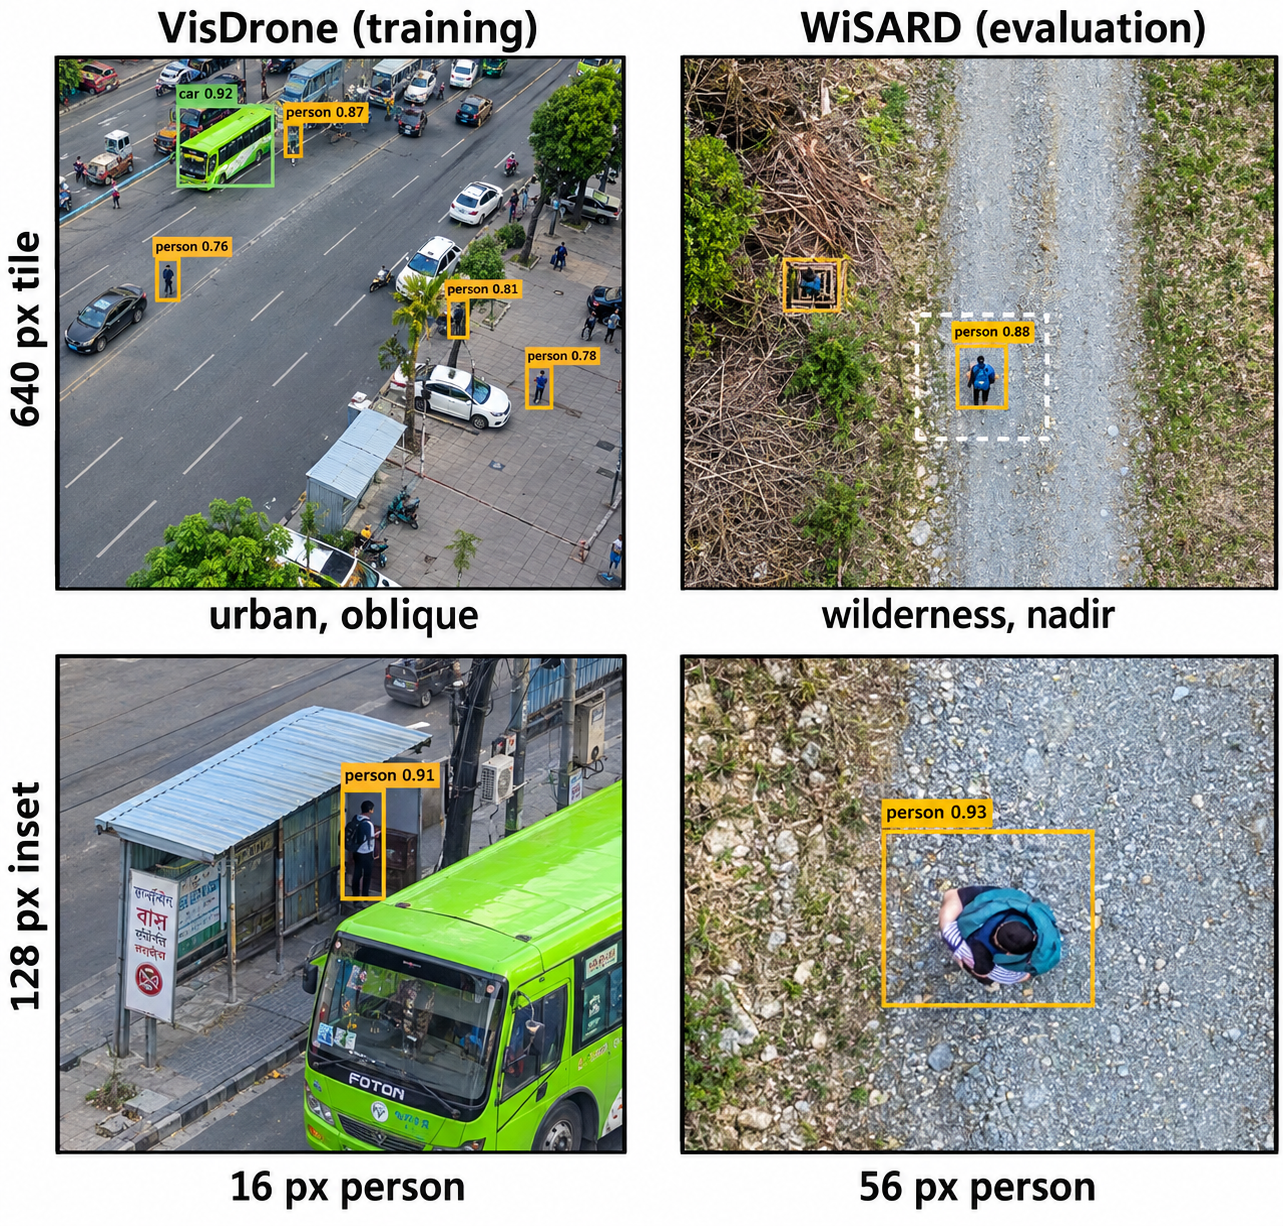
\includegraphics[width=0.9\columnwidth]{fig3_domain_shift.png}
\caption{The domain shift, at identical scale. Top: 640\,px tiles cut at native
resolution, with annotated persons boxed. Bottom: the same 128\,px window around
a person of each corpus's median size, a 16\,px oblique figure against a 56\,px
top-down form.}
\label{fig:shift}
\end{figure}

\subsection{The Shift Is Toward Larger, Nadir Targets}

Fig.~\ref{fig:shift} shows the two corpora in identical 640\,px tile space,
differing in the opposite direction to the one the small-object literature
suggests. VisDrone training persons average 20.88\,px across 218,769 instances,
with 74.8\% between 8 and 32\,px, while WiSARD persons average 67.30\,px across
8,345 instances, with 79.5\% at or above 32\,px. The bounding-box aspect ratio
shifts from 2.00 to 1.46, consistent with a change from oblique street-level
views, where a standing person is an upright figure, to the near-nadir view of a
wilderness overflight, where the same person is a compact top-down blob. The
cross-domain target is therefore roughly three times larger than the training
distribution, not smaller.

\subsection{Reducing the Inference Input Helps, but Not for the Expected Reason}

The model is fully convolutional, so apparent object size can be changed at
inference by altering the input resolution, with no retraining. Sweeping it from
640 down to 160\,px gives a smooth inverted-U in cross-domain accuracy, peaking
at 320\,px, where AP@0.5 reaches 0.3291 against 0.2567 at the native 640. A
paired sequence-level bootstrap puts the difference at $+0.068$ with a 95\%
interval of $[0.019, 0.117]$, significant between 512 and 320\,px and
indistinguishable from zero at 256\,px and below. It survives Bonferroni
correction across the seven comparisons (marginally at 320\,px, $+0.002$,
against $+0.028$ at 512).

The mechanism is not the one the size measurement suggests. Decomposing the
change shows true positives rise only from 5,081 to 5,202 and the recall ceiling
moves from 0.609 to 0.623, while false positives fall from 204,087 to 109,493, a
46\% reduction. Halving the inference resolution does not reveal people the
detector was missing, it stops it asserting people who are not there. The gain
is real, significant and free, but it is a precision effect.

Requiring agreement between 640 and 320\,px removes 47--64\% of false positives
but also 7--9\% of true positives, and no consensus variant beats single-scale
320 (0.3269 against 0.3296), so what is lost at reduced resolution is not only
spurious.

\subsection{What Target-Domain Data Recovers}

Fine-tuning on 31 wilderness sequences and testing on 5 the model never saw
raises person AP@0.5 from 0.0746 to 0.4575, and recall from 0.120 to 0.459, a
factor of 6.1. Zero-shot on this subset scores 0.0746, against 0.2567 over all
38 sequences, so these five are harder than the corpus average and the
multiplier is specific to them.

The amount of target data needed saturates. We repeated the fine-tune at 1, 2,
4, 8, 16 and 31 training sequences under three seeds. Mean person AP@0.5 is
0.082, 0.189, 0.372, 0.369, 0.456 and 0.449. The $N=31$ point carries no seed
variance by construction: thirty-one sequences exhaust the pool, the three seed
splits are byte-identical, and deterministic training returns one number three
times. Budget runs trained for 15 epochs while the headline fine-tune
early-stopped at epoch 21 of 40, which is why the curve reads 0.449 at 31
sequences against the headline's 0.4575. Below that, spread matters more than
mean: the seeds range over 0.347 at $N=4$, because per-sequence annotation
counts run from 0 to 1,122 and a small draw is decided by which sequences it
contains. At sixteen the spread collapses to 0.035 and the mean matches the full
set, so at this sample size further labelling brings no measurable gain, and a
modest annotation campaign buys most of the available recovery.

\begin{figure}[!t]
\centering
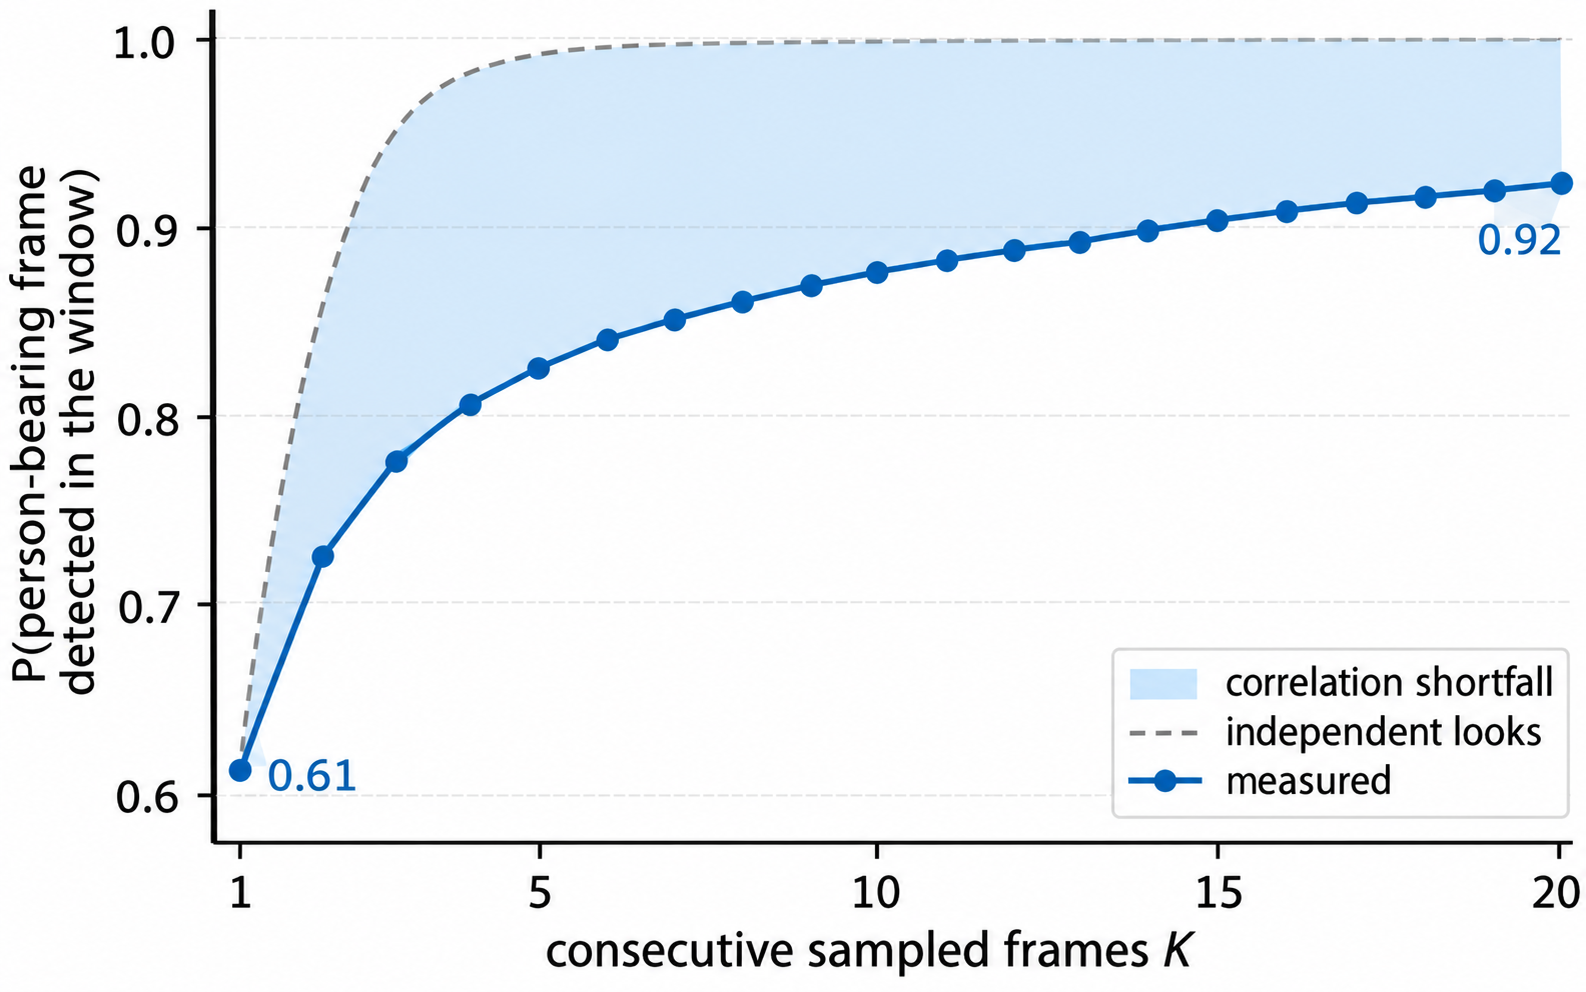
\includegraphics[width=0.95\columnwidth]{fig4_encounter.png}
\caption{Encounter-level detection against window length $K$, with the
independent-looks bound above it. The shaded band is the shortfall between the
two.}
\label{fig:encounter}
\end{figure}

\subsection{Repeated Coverage Recovers Part of the Shortfall}

Per-frame recall is not what a search cares about. An aircraft passes over the
same ground repeatedly and a person need only be found once. WiSARD carries no
track identifiers, so we measure frame presence within a flight. A frame is
positive when any tile holds an annotated person and detected when any tile
yields a true positive above the operating threshold. A window of $K$
consecutive positive frames counts as detected if any frame in it is. The
windows come from ground truth, so this bounds what repetition can recover
rather than describing a live search.

This study is scored at 320\,px with an operating threshold of 0.1515, the
reduced-resolution row of Table~\ref{tab:main}, not the 640\,px headline. Over
1,703 positive frames in 32 sequences, a single frame is detected with
probability 0.609 [.472--.742], rising to 0.923 [.799--.997] over 20 consecutive
sampled frames (Fig.~\ref{fig:encounter}). Tiles were built at every tenth
frame, so $K$ counts sampled frames about a third of a second apart at 30\,fps,
making $K=20$ roughly 6.7\,s of flight. The curve sits below the
independent-looks bound, by up to 0.178 at $K=4$, because consecutive views
share pose, illumination and background.

\subsection{Export Precision on the Target Hardware}

Latency was measured on the Pi 4 at four threads as described in
Section~\ref{sec:ondevice}, so every figure here excludes non-maximum
suppression and bounds deployed cost from below. TFLite FP32 runs at 495\,ms and
the hybrid-integer export at 761\,ms, both within 0.72 percentage points of the
PyTorch reference on all-class mAP@0.5, not comparable to the person-only
numbers above. That parity rules out a preprocessing mismatch. Identical
letterbox, channel order and input scaling give faithful results everywhere
except the integer-activation path. Full-integer quantisation, where activations
as well as weights become integers \cite{jacob2018,gholami2022}, runs at
410\,ms, a 1.21$\times$ speed-up, and costs 12.80 percentage points. The split
between the two integer exports locates the fragility in the activations rather
than the weights, what a Softmax inside the distribution-focal-loss head would
produce, and an independent report reaches the same attribution \cite{chen2026}.
The hybrid variant is slower and no more accurate, so it is dominated outright.

\section{Discussion}
\label{sec:discussion}

The false-positive result has an explanation in the class balance reported
above. The detector was trained almost entirely on evidence that something is
present, then asked to spend deployment deciding that nothing is. Retraining
identically on every negative tile VisDrone can supply lifts the negative
fraction from 1.33\% to 9.55\%, but the benefit depends on where recall is
fixed. Cross-domain false positives at matched recall change by $+12.0$,
$-6.6$, $-32.9$, $-41.9$ and $-32.6$ percent at recall 0.10 through 0.50, so the
lowest recall point moves the wrong way. AP@0.5 rises from 0.2570 to 0.2784 with
the recall ceiling unchanged within 0.006. Three bounds apply. This is one
baseline checkpoint against one control, so there is no seed axis. The corpus
exhausts at 9.55\% against WiSARD's 85.8\%. The same comparison at epoch 50
shows no benefit, placing the effect in late-training divergence.

The same recall-first framing explains why full-integer quantisation is a poor
trade here. Our 12.8-point cost for a 1.21$\times$ speed-up matches the
nano-scale figure in \cite{rey2025}, against 5.8 points for a small-scale model,
and on the device the trade is unnecessary too. Moving the deployed payload to
floating point raises median inference from 645 to 772\,ms, a factor of 1.20,
yet across sessions of 6 to 17 minutes both precisions sustain the same
0.91--1.20\,s$^{-1}$ end-to-end. Capture, tiling and encoding set the pace, so a
20\% slower model is absorbed rather than paid for, and recovering the 12.8
points cost no throughput.

Throughput depends on what is timed, and on what governor is set. Over stored
frames a single 416\,px tile costs 171\,ms under \texttt{ondemand}, against
\texttt{performance} behind the 640\,px figures, so the two are not a
like-for-like pair. The four tiles covering a frame spend 0.69\,s in the
interpreter and the benchmark completes 1.33 sets per second, while the full
service, which also captures and encodes, runs at the rates above. Whether
either suffices depends on airspeed and altitude, which we have not measured,
and the 320\,px gain is unconfirmed on-device. The operating point must also be
set deliberately. Across all 37,058 tiles the conventional 0.25 threshold
recovers 30.1\% of annotated people against 38.7\% at 0.10, so the inherited
default discards 28\% of available recall for 0.18 more false positives per tile
and no latency cost.

One factor cuts across every number above. Scoring the periodic checkpoints of
both baseline seeds against WiSARD shows cross-domain accuracy is not monotone
in training: it peaks at epochs 70 and 60, at AP@0.5 0.3149 and 0.2966, then
falls to 0.2570 and 0.2532 by epoch 120, a relative loss of 18.4\% and 14.6\%,
while in-domain validation rises throughout. The checkpoint ordinary practice
selects is not the one that transfers, so our reported figures, taken at epoch
120, are pessimistic by roughly a sixth and bound the gap a target-aware
stopping rule would leave. This also explains why the negative-fraction control
helps only late: the extra negatives mostly prevent this decline rather than
raising the peak.

\section{Limitations}
\label{sec:limits}

Scale and viewpoint shift together and our experiments cannot separate them.
Reducing the inference input changes apparent object size while holding the
ground footprint fixed, not ground-sample-distance matching, which would need
source frames we no longer hold. The residual gap mixes viewpoint, pose, terrain
and illumination.

Statistical support rests on resampling 38 flight sequences, correct for
correlated video but small, so the intervals in Table~\ref{tab:main} are wide.
New configurations were trained at one seed, except the headline rows, the
budget curve at three and the epoch sweep at two. The fine-tuning multiplier is
a point estimate, and neither it nor the negative-fraction result is re-derived
from the epoch-70 checkpoint.

Most importantly, nothing here is flight-validated: every accuracy figure comes
from recorded imagery, and every on-device figure from a Pi 4 on a desk. We make
no claim about vibration, rolling shutter, motion blur at airspeed, throttling
under a fairing, or latency in a real search.

The benchmark has known weaknesses: WiSARD shows targets in bright clothing in
open terrain \cite{manzini2023}, while real missing persons typically seek
shelter, so absolute accuracy here should be read as optimistic. We evaluate
visible-spectrum only; a thermal channel is measurably stronger here, and
thermal tracking systems for search and rescue already exist
\cite{yeom2024a,yeom2024b}, the obvious upgrade for a capable airframe.

\section{Conclusion}
\label{sec:conclusion}

A nano-scale detector trained on urban aerial imagery loses roughly a third of
its person-detection accuracy over wilderness. Tiled training bounds that loss,
worth at most 5.7$\times$ over a resize-only control scored with inference-time
slicing, and the shift is toward larger, near-nadir targets. Halving the
inference input recovers 0.068 AP@0.5 by suppressing 46\% of false positives,
not by finding more people, and extra negative tiles cut a further third at
mid-range matched recall. Repeated coverage lifts encounter-level detection from
0.609 to 0.923. The rest is an appearance gap only target-domain data closes,
with fine-tuning recovering a factor of 6.1 and saturating near sixteen labelled
sequences.

For teams deploying this class of system: tiling is not optional, inference
resolution, decision threshold, negative sampling and stopping epoch are free
and underused knobs, and sixteen labelled target-domain sequences buy more than
any of them.

Three extensions follow: a flight trial of the Pi 4 payload to measure motion
blur, throttling and latency at airspeed; a target-aware stopping rule,
re-deriving the fine-tuning and negative-fraction results from that checkpoint;
and a ground-sample-distance matched evaluation separating size and viewpoint.
The airframe has room to develop alongside them: RF telemetry would extend its
range and autonomy, together with work on endurance and precise navigation, and
running the detector in the loop with the flight controller would let the
aircraft react to what it spots while it is still overhead.

\begin{thebibliography}{99}

\bibitem{elashaal2024}
Z. A. Elashaal, Y. H. Lamin, M. K. Elfandi, and A. A. Eluheshi, ``Autonomous
search and rescue drone,'' \emph{Libyan Journal of Informatics}, vol. 1, no. 1,
pp. 1--17, 2024.

\bibitem{lago2024}
A. Lago, S. Patel, and A. Singh, ``Low-cost real-time aerial object detection
and gps location tracking pipeline,'' \emph{ISPRS Open Journal of Photogrammetry
and Remote Sensing}, vol. 13, p. 100069, 2024.

\bibitem{stasik2025}
J. Stasik and T. Szandala, ``An autonomous drone for avalanche search and
rescue: Integrating ardupilot and tracking-beacon detection,'' \emph{IEEE
Access}, vol. 13, pp. 130758--130769, 2025.

\bibitem{akyon2022}
F. C. Akyon, S. O. Altinuc, and A. Temizel, ``Slicing aided hyper inference and
fine-tuning for small object detection,'' in \emph{2022 IEEE International
Conference on Image Processing (ICIP)}, 2022, pp. 966--970.

\bibitem{chen2026}
P. Chen, H. Sa, Y. Hu, Y. Cheng, and J. Wang, ``Sdd-yolo: A small-target
detection framework for ground-to-air anti-uav surveillance with edge-efficient
deployment,'' 2026, arXiv:2603.25218.

\bibitem{song2025}
Z. Song, Y. Yan, Y. Cao, S. Jin, F. Qi, Z. Li, T. Lei, L. Chen, Y. Jing, J. Xia,
X. Liang, and G. Lu, ``An infrared dataset for partially occluded person
detection in complex environment for search and rescue,'' \emph{Scientific
Data}, vol. 12, no. 1, 2025.

\bibitem{sambolek2024}
S. Sambolek and M. Ivasic-Kos, ``Person detection and geolocation estimation in
uav aerial images: An experimental approach,'' in \emph{Proceedings of the 13th
International Conference on Pattern Recognition Applications and Methods
(ICPRAM)}, 2024, pp. 785--792.

\bibitem{ahn2023}
H. Ahn, T. Chen, N. Alnaasan, A. Shafi, M. Abduljabbar, H. Subramoni, and
D. K. Panda, ``Performance characterization of using quantization for dnn
inference on edge devices: Extended version,'' 2023, arXiv:2303.05016.

\bibitem{rey2025}
L. Rey, A. M. Bernardos, A. D. Dobrzycki, D. Carrami\~{n}ana, L. Bergesio,
J. A. Besada, and J. R. Casar, ``A performance analysis of you only look once
models for deployment on constrained computational edge devices in drone
applications,'' \emph{Electronics}, vol. 14, no. 3, p. 638, 2025.

\bibitem{humes2023}
E. Humes, M. Navardi, and T. Mohsenin, ``Squeezed edge yolo: Onboard object
detection on edge devices,'' 2023, arXiv:2312.11716.

\bibitem{alqahtani2024}
D. K. Alqahtani, M. A. Cheema, M. A. Rodriguez, and A. N. Toosi, ``A
comprehensive evaluation of deep learning object detection models on
heterogeneous edge devices,'' 2024, arXiv:2409.16808.

\bibitem{zell2026}
S. E. Zell, T. Schneidereit, A. F\"{u}genschuh, and M. Breu\ss{}, ``Autonomous
unmanned aircraft systems for enhanced search and rescue of drowning swimmers:
Image-based localization and mission simulation,'' 2026, arXiv:2604.18088.

\bibitem{sachdeva2025}
A. Sachdeva, D. Ganeshkumar, J. E. Gallagher, T. Treat, and E. J. Oughton,
``Evaluating an adaptive multispectral turret system for autonomous tracking
across variable illumination conditions,'' 2025, arXiv:2512.22263.

\bibitem{zhang2025}
X. Zhang, Y. Feng, N. Wang, G. Lu, and S. Mei, ``Aerial person detection for
search and rescue: Survey and benchmarks,'' \emph{Journal of Remote Sensing},
vol. 5, 2025.

\bibitem{zhu2021}
P. Zhu, L. Wen, D. Du, X. Bian, H. Fan, Q. Hu, and H. Ling, ``Detection and
tracking meet drones challenge,'' \emph{IEEE Transactions on Pattern Analysis
and Machine Intelligence}, 2021.

\bibitem{broyles2022}
D. Broyles, C. R. Hayner, and K. Leung, ``WiSARD: A labeled visual and thermal
image dataset for wilderness search and rescue,'' in \emph{2022 IEEE/RSJ
International Conference on Intelligent Robots and Systems (IROS)}, Kyoto,
Japan, 2022, pp. 9467--9474.

\bibitem{manzini2023}
T. Manzini and R. Murphy, ``Open problems in computer vision for wilderness sar
and the search for patricia wu-murad,'' 2023, arXiv:2307.14527.

\bibitem{fraternali2025}
P. Fraternali, L. Morandini, and R. Motta, ``Enhancing search and rescue
missions with uav thermal video tracking,'' \emph{Remote Sensing}, vol. 17,
no. 17, p. 3032, 2025.

\bibitem{farrell2025}
S. Farrell, C. Li, and H. I. Christensen, ``Glide: A coordinated aerial-ground
framework for search and rescue in unknown environments,'' 2025,
arXiv:2509.14210.

\bibitem{jacob2018}
B. Jacob, S. Kligys, B. Chen, M. Zhu, M. Tang, A. Howard, H. Adam, and
D. Kalenichenko, ``Quantization and training of neural networks for efficient
integer-arithmetic-only inference,'' in \emph{2018 IEEE/CVF Conference on
Computer Vision and Pattern Recognition (CVPR)}, 2018, pp. 2704--2713.

\bibitem{wu2020}
H. Wu, P. Judd, X. Zhang, M. Isaev, and P. Micikevicius, ``Integer quantization
for deep learning inference: Principles and empirical evaluation,'' 2020,
arXiv:2004.09602.

\bibitem{gholami2022}
A. Gholami, S. Kim, Z. Dong, Z. Yao, M. W. Mahoney, and K. Keutzer, ``A survey
of quantization methods for efficient neural network inference,'' in
\emph{Low-Power Computer Vision}.\ Chapman and Hall/CRC, 2022, pp. 291--326.

\bibitem{boddu2025}
S. Boddu and A. Mukherjee, ``Efficient edge deployment of quantized yolov4-tiny
for aerial emergency object detection on raspberry pi 5,'' 2025,
arXiv:2506.09300.

\bibitem{shamrai2025}
M. Shamrai, ``YOLOv8s-VisDrone,'' 2025, Hugging Face model card,
\url{https://huggingface.co/mshamrai/yolov8s-visdrone}.

\bibitem{yeom2024a}
S. Yeom, ``Thermal image tracking for search and rescue missions with a
drone,'' \emph{Drones}, vol. 8, no. 2, p. 53, 2024.

\bibitem{yeom2024b}
------, ``Multi-rotor drone-based thermal target tracking with track segment
association for search and rescue missions,'' \emph{Drones}, vol. 8, no. 11,
p. 689, 2024.

\end{thebibliography}

\end{document}